\section{FDP  Class Reference}
\label{classFDP}\index{FDP@{FDP}}
A dynamic programming approach to nonholonomic planning, as proposed by Barraquand, Latombe, Algorithmica 10:6, pp. 121-155, 1993. 


{\tt \#include $<$fdp.h$>$}

Inheritance diagram for FDP::\begin{figure}[H]
\begin{center}
\leavevmode
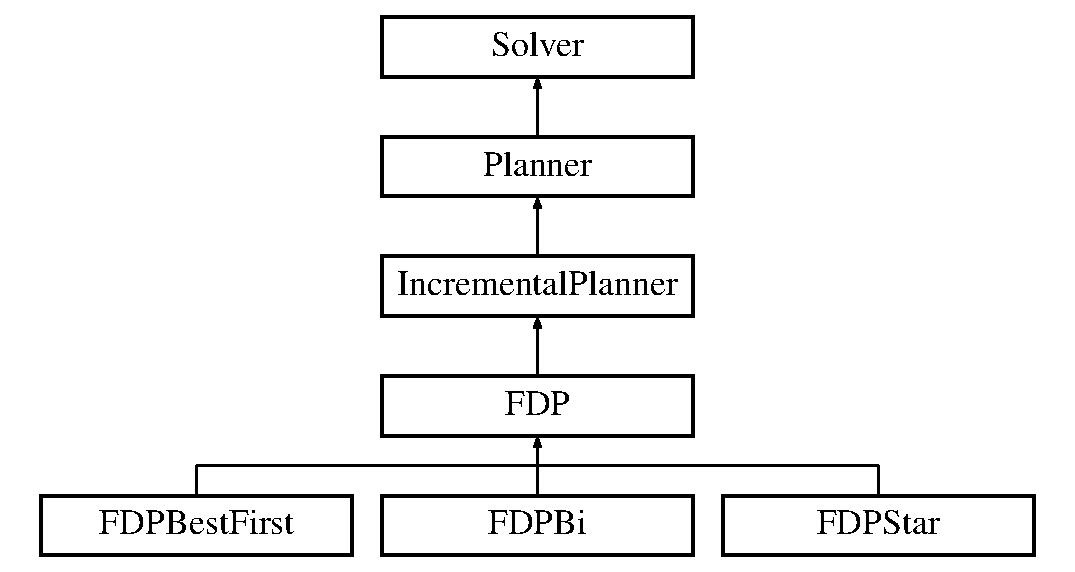
\includegraphics[height=5cm]{classFDP}
\end{center}
\end{figure}
\subsection*{Public Methods}
\begin{CompactItemize}
\item 
{\bf FDP} ({\bf Problem} $\ast$problem)
\begin{CompactList}\small\item\em A constructor that initializes data members.\item\end{CompactList}\item 
{\bf $\sim$FDP} ()
\begin{CompactList}\small\item\em Empty destructor.\item\end{CompactList}\item 
virtual void {\bf Reset} ()
\begin{CompactList}\small\item\em Reset the planner.\item\end{CompactList}\item 
virtual bool {\bf Plan} ()
\begin{CompactList}\small\item\em Attempt to solve an Initial-Goal query by growing an FDP tree.\item\end{CompactList}\end{CompactItemize}
\subsection*{Public Attributes}
\begin{CompactItemize}
\item 
int {\bf Satisfied\-Count}
\begin{CompactList}\small\item\em Number of times the collision checker has been called.\item\end{CompactList}\end{CompactItemize}
\subsection*{Protected Methods}
\begin{CompactItemize}
\item 
virtual double {\bf Search\-Cost} (double initcost, {\bf MSLNode} $\ast$\&n, {\bf MSLNode} $\ast$\&nn)
\item 
virtual vector$<$int$>$ {\bf State\-To\-Indices} (const {\bf MSLVector} \&x)
\item 
virtual {\bf MSLVector} {\bf Indices\-To\-State} (const vector$<$ int $>$ \&indices)
\end{CompactItemize}
\subsection*{Protected Attributes}
\begin{CompactItemize}
\item 
priority\_\-queue$<${\bf MSLNode}$\ast$,vector$<${\bf MSLNode}$\ast$$>$,{\bf MSLNode\-Greater}$>$ {\bf Q}
\begin{CompactList}\small\item\em Priority queue of nodes.\item\end{CompactList}\item 
{\bf Multi\-Array}$<$int$>$$\ast$ {\bf Grid}
\begin{CompactList}\small\item\em A quantized state space.\item\end{CompactList}\item 
vector$<$int$>$ {\bf Grid\-Dimensions}
\begin{CompactList}\small\item\em Dimensions for the grid.\item\end{CompactList}\item 
int {\bf Grid\-Default\-Resolution}
\begin{CompactList}\small\item\em Default size for each axis of the grid.\item\end{CompactList}\item 
{\bf MSLVector} {\bf Quantization}
\begin{CompactList}\small\item\em The quantized step size for each axis (computed automatically).\item\end{CompactList}\end{CompactItemize}


\subsection{Detailed Description}
A dynamic programming approach to nonholonomic planning, as proposed by Barraquand, Latombe, Algorithmica 10:6, pp. 121-155, 1993.

Forward Dynamic Programming, as proposed by Barraquand, Latombe,  Algorithmica 10:6, pp. 121-155, 1993. The solutions should be optimized  with respect to time, although problems can be caused by quantization  errors.

When an instance is constructed, a grid is initialized and each element of checked for collision. The test point for collision is the center of the cell. The current version does not use distance computations; therefore, a large value for Planner\-Delta\-T might cause collisions to be missed.

Make sure that Planner\-Delta\-T is large enough to allow the state to move from one cell to another without in a single step. For example, if the quantization leads to a grid boundary every 2.0 units, then Planner\-Delta\-T could be set to cause the state to change by 3.0 units.

Grid\-Dimensions sets the resolution of the grid and can be read from a file. For high-dimensional problems an error message may occur due to a grid that is too large. To enable larger grids, set the Max\-Size to a desirable size in the {\bf Multi\-Array} {\rm (p.\,\pageref{classMultiArray})} class (in {\bf marray.C}). 



\subsection{Constructor \& Destructor Documentation}
\index{FDP@{FDP}!FDP@{FDP}}
\index{FDP@{FDP}!FDP@{FDP}}
\subsubsection{\setlength{\rightskip}{0pt plus 5cm}FDP::FDP ({\bf Problem} $\ast$ {\em problem})}\label{classFDP_a0}


A constructor that initializes data members.

\index{FDP@{FDP}!~FDP@{$\sim$FDP}}
\index{~FDP@{$\sim$FDP}!FDP@{FDP}}
\subsubsection{\setlength{\rightskip}{0pt plus 5cm}FDP::$\sim$FDP ()\hspace{0.3cm}{\tt  [inline]}}\label{classFDP_a1}


Empty destructor.



\subsection{Member Function Documentation}
\index{FDP@{FDP}!IndicesToState@{IndicesToState}}
\index{IndicesToState@{IndicesToState}!FDP@{FDP}}
\subsubsection{\setlength{\rightskip}{0pt plus 5cm}{\bf MSLVector} FDP::Indices\-To\-State (const vector$<$ int $>$ \& {\em indices})\hspace{0.3cm}{\tt  [protected, virtual]}}\label{classFDP_b2}


\index{FDP@{FDP}!Plan@{Plan}}
\index{Plan@{Plan}!FDP@{FDP}}
\subsubsection{\setlength{\rightskip}{0pt plus 5cm}bool FDP::Plan ()\hspace{0.3cm}{\tt  [virtual]}}\label{classFDP_a3}


Attempt to solve an Initial-Goal query by growing an FDP tree.



Reimplemented from {\bf Planner} {\rm (p.\,\pageref{classPlanner_a4})}.

Reimplemented in {\bf FDPBi} {\rm (p.\,\pageref{classFDPBi_a3})}.\index{FDP@{FDP}!Reset@{Reset}}
\index{Reset@{Reset}!FDP@{FDP}}
\subsubsection{\setlength{\rightskip}{0pt plus 5cm}void FDP::Reset ()\hspace{0.3cm}{\tt  [virtual]}}\label{classFDP_a2}


Reset the planner.



Reimplemented from {\bf Planner} {\rm (p.\,\pageref{classPlanner_a2})}.

Reimplemented in {\bf FDPBi} {\rm (p.\,\pageref{classFDPBi_a2})}.\index{FDP@{FDP}!SearchCost@{SearchCost}}
\index{SearchCost@{SearchCost}!FDP@{FDP}}
\subsubsection{\setlength{\rightskip}{0pt plus 5cm}double FDP::Search\-Cost (double {\em initcost}, {\bf MSLNode} $\ast$\& {\em n}, {\bf MSLNode} $\ast$\& {\em nn})\hspace{0.3cm}{\tt  [protected, virtual]}}\label{classFDP_b0}




Reimplemented in {\bf FDPStar} {\rm (p.\,\pageref{classFDPStar_b0})}, and {\bf FDPBest\-First} {\rm (p.\,\pageref{classFDPBestFirst_b0})}.\index{FDP@{FDP}!StateToIndices@{StateToIndices}}
\index{StateToIndices@{StateToIndices}!FDP@{FDP}}
\subsubsection{\setlength{\rightskip}{0pt plus 5cm}vector$<$ int $>$ FDP::State\-To\-Indices$<$int$>$ (const {\bf MSLVector} \& {\em x})\hspace{0.3cm}{\tt  [protected, virtual]}}\label{classFDP_b1}




\subsection{Member Data Documentation}
\index{FDP@{FDP}!Grid@{Grid}}
\index{Grid@{Grid}!FDP@{FDP}}
\subsubsection{\setlength{\rightskip}{0pt plus 5cm}{\bf Multi\-Array}$<$ int $>$ $\ast$ FDP::Grid\hspace{0.3cm}{\tt  [protected]}}\label{classFDP_n1}


A quantized state space.

\index{FDP@{FDP}!GridDefaultResolution@{GridDefaultResolution}}
\index{GridDefaultResolution@{GridDefaultResolution}!FDP@{FDP}}
\subsubsection{\setlength{\rightskip}{0pt plus 5cm}int FDP::Grid\-Default\-Resolution\hspace{0.3cm}{\tt  [protected]}}\label{classFDP_n3}


Default size for each axis of the grid.

\index{FDP@{FDP}!GridDimensions@{GridDimensions}}
\index{GridDimensions@{GridDimensions}!FDP@{FDP}}
\subsubsection{\setlength{\rightskip}{0pt plus 5cm}vector$<$ int $>$ FDP::Grid\-Dimensions\hspace{0.3cm}{\tt  [protected]}}\label{classFDP_n2}


Dimensions for the grid.

\index{FDP@{FDP}!Q@{Q}}
\index{Q@{Q}!FDP@{FDP}}
\subsubsection{\setlength{\rightskip}{0pt plus 5cm}priority\_\-queue$<$ {\bf MSLNode} $\ast$,vector$<$ {\bf MSLNode} $\ast$$>$,{\bf MSLNode\-Greater} $>$ FDP::Q\hspace{0.3cm}{\tt  [protected]}}\label{classFDP_n0}


Priority queue of nodes.

\index{FDP@{FDP}!Quantization@{Quantization}}
\index{Quantization@{Quantization}!FDP@{FDP}}
\subsubsection{\setlength{\rightskip}{0pt plus 5cm}{\bf MSLVector} FDP::Quantization\hspace{0.3cm}{\tt  [protected]}}\label{classFDP_n4}


The quantized step size for each axis (computed automatically).

\index{FDP@{FDP}!SatisfiedCount@{SatisfiedCount}}
\index{SatisfiedCount@{SatisfiedCount}!FDP@{FDP}}
\subsubsection{\setlength{\rightskip}{0pt plus 5cm}int FDP::Satisfied\-Count}\label{classFDP_m0}


Number of times the collision checker has been called.



The documentation for this class was generated from the following files:\begin{CompactItemize}
\item 
{\bf fdp.h}\item 
{\bf fdp.C}\end{CompactItemize}
